\section{Zielsetzung}
\label{sec:Zielsetzung}

In diesem Versuch sollen Brechungsindizes eines Glasprismas für verschiedene Wellenlängen mithilfe von Sprektrallinien bestimmt werden.
Ebenso soll die Dispersionskurve bestimmt werden.

\section{Theorie}
\subsection{Brechung und Dispersion}
Bewegt sich Licht in einem Medium $1$ mit Brechungsindex $n_1$ und trifft unter dem Winkel $\alpha_1$
auf die Grenzfläche eines Mediums $2$ mit Brechungsindex $n_2$, so kommt es zur Brechung.
Das heißt, dass das Licht mit einem Winkel $\alpha_1$ auf die Grenzfläche trifft und sich daraufhin mit einem
Winkel $\alpha_2$ ausbreitet.
Wie in Abbildung \ref{fig:brech} zu sehen ist, werden beide Winkel dabei zum Lot der Grenzfläche gemessen.
\begin{figure}[H]
  \centering
  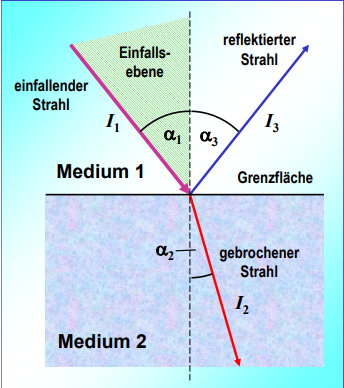
\includegraphics[scale=0.7]{Text/Bilder/Brechung2.PNG}
  \caption{Schematische Darstellung der Brechung an einer Grenzfläche \cite[948]{sample3}}
  \label{fig:brech}
\end{figure}
Mithilfe des Huygensschen Prinzips, welches besagt, dass jeder jeder Punkt einer Welle als Ursprung einer Elementarwelle angesehen werden kann,
kann mit
\begin{equation}
 n := \frac{v_1}{v_2} \label{eqn:LiM}
\end{equation}
\begin{center}
 \tiny {($v_i \: \hat{=} \:\text{Geschwindigkeit des Lichts im Medium $i$}$)}
\end{center}
für die Brechung folgender Zusammenhang hergeleitet werden:
\begin{equation}
  \frac{\sin{\alpha_1}}{\sin{\alpha_2}} = \frac{n_2}{n_1} = n \text{.} \label{eqn:SBG}
\end{equation}
Der in Gleichung \eqref{eqn:SBG} beschriebende Zusammenhang ist als Snellius Snellius-Brechungsgesetz bekannt.
Bei genauerer Betrachtung stellt sich heraus, dass der Brechungsindex $n$ von der Wellenlänge $\lambda$ abhängt.
Es gilt somit $n=f(\lambda)$. Dieser Zusammenhang wird als Dispersion bezeichnet. $f(\lambda)$ ist die sogegannte Dispersionskurve.
Der genaue Zusammenhang wird in Kapitel \ref{sec:AdD} erläuert.

\subsection{Ableitung der Dispersionsgleichung}\label{sec:AdD}
Gesucht ist nun ein Zusammenhang zwischen dem Brechungsindex $n$ und $\lambda$. Dieser Zusammenhang wird durch die Dispersionsgleichung beschrieben.
Um diese zu erhalten, muss die Annahme, dass Materie ein elektrisch neutrales Kontinuum ist, verworfen und die elektrisch geladenen Bestandteile, das heißt
Elektronen und Ionenrümpfe, der Materie berücksichtigt werden. Diese werden durch das elektromagnetische Wechselfeld des Lichts zu Schwingungen angeregt.
Dabei können Resonanzerscheinungen auftreten, die mithilfe dieses Modells nicht vollständiges beschrieben werden können. Aus diesem Grund werden in diesem
Experiment Wellenlängen betrachtet, die hinreichend weit entfernt von der Resonanzwellenlänge sind.
Ebenso ist diese Modellvorstellung der Wechselwirkung zwischen Materie und Strahlung  nicht für Wellenlängen unterhalb des sichtbaren Spektrum gültig,
da es dort verstärkt zu quantenmechanischen Effekten kommt.
Nach einer längeren Rechnung kann, unter der Annahme, dass die schwingenden Teilchen einen elektrischen Dipol darstellen, mit der Maxwellschen Relation
$\epsilon=n^2$ folgender Zusammenhang gefunden werden:
\begin{equation}
n^2(\lambda)=1+\sum_h\frac{N_hq^2_h}{4\pi^2 c^2\epsilon_0 m_h}\frac{\lambda^2\lambda^2_h}{\lambda^2-\lambda^2_h}\text{.}\label{eqn:n^2}
\end{equation}
\begin{center}
 \tiny {($N_h \: \hat{=} \:\text{Anzahl der Teilchen pro Volumeneinheit}$, $m_h \: \hat{=} \:\text{teilchenmasse}$, $q_h \: \hat{=} \:\text{Ladungen}$, $\lambda_h \: \hat{=} \:\text{Resonanzwellenlänge}$ )}
\end{center}

Liegt lediglich eine Resonanzfrequenz vor, so kann dabei unter $\lambda \gg \lambda_1$ und $\lambda \ll \lambda_1$ unterschieden werden.
Für den Fall $\lambda \gg \lambda_1$ kann die Gleichung \eqref{eqn:n^2} wie folgt geschrieben werden:
\begin{align}
n^2(\lambda)&=1+\frac{N_1 q_1^2 \lambda_1^2}{4\pi^2 c^2 \epsilon_0 m_1}\left(1+\left(\frac{\lambda_1}{\lambda}\right)^2+\left(\frac{\lambda_1}{\lambda}\right)^4+\ldots\right)\nonumber\\
			&=A_0+\frac{A_2}{\lambda^2}+\frac{A_4}{\lambda^4}+\ldots \label{eq:n^2 für l>>l1} \text{,}
\end{align}
während für den Fall $\lambda \ll \lambda_1$ gilt:
\begin{align}
n^2(\lambda)&=1-\frac{N_1 q_1^2 }{4\pi^2 c^2 \epsilon_0 m_1}\left(\lambda^2+\frac{\lambda^4}{\lambda_1^2}+\frac{\lambda^6}{\lambda_1^4}+\ldots\right)\nonumber\\
			&=1-A_2^\prime\lambda^2-A_4^\prime\lambda^4-\ldots \label{eq:n^2 für l<<l1}
\end{align}
Die Kurvenverläufe sind in den Abbildungen \ref{fig:case1} und \ref{fig:case2} dargestellt.\newline \newline
\begin{minipage}{0.45\textwidth}
\begin{figure}[H]
  \centering
  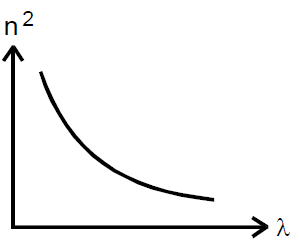
\includegraphics[scale=0.7]{Text/Bilder/case1.png}
  \caption{$\lambda \ll \lambda_1$ \cite[22]{sample}.}
  \label{fig:case1}
\end{figure}
\end{minipage}
%\vline{}
\begin{minipage}{0.45\textwidth}
\begin{figure}[H]
  \centering
  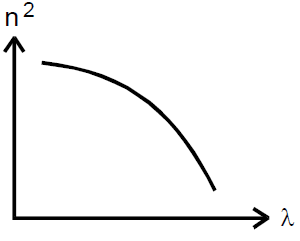
\includegraphics[scale=0.7]{Text/Bilder/case2.png}
  \caption{$\lambda \gg \lambda_1$ \cite[22]{sample}.}
  \label{fig:case2}
\end{figure}
\end{minipage}
\newline
Den Abbildungen \ref{fig:case1} und \ref{fig:case2} ist zu entnehmen, dass der Brechungsindex mit zunehmender Wellenlänge abnimmt. Es liegt daher Dispersion vor.
Der umgekehrte Fall – die Zunahme von n mit wachsenden $\lambda$ – wird dagegen als anomale Dispersion bezeichnet.


\subsection{Brechung am Prisma}\label{sec:brech}
Fällt Licht auf ein Prisma, so wird dieses, sofern es nicht senkrecht auf dieses trifft, zwei mal gebrochen, wie in Abbildung \ref{fig:BaP} zu sehen ist..
\begin{figure}[H]
  \centering
  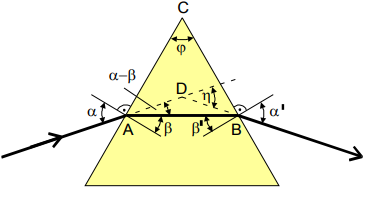
\includegraphics[scale=0.7]{Text/Bilder/Brechung3.PNG}
  \caption{Symetrischer Strahlengang durch ein Prisma \cite[23]{sample}}
  \label{fig:BaP}
\end{figure}
Aus geometrischen überlegungen sowieso der Annahme, dass durch den symmetrischen Strahlengang die Beziehungen $\alpha=\alpha'$ sowie $\beta=\beta'$ gelten,   folgt:
\begin{equation}
  \eta=2 \left(\alpha-\beta \right)
\end{equation}
sowie
\begin{align}
  \alpha &= \frac{\phi + \eta}{2} \\
  \beta  &= \frac{\phi}{2} \text{.}
\end{align}
Mit dem Snelliusschen Brechungsgesetz \eqref{eqn:SBG} ergibt sich somit für den Brechungsindex:
\begin{equation}
n = \frac{\sin\frac{\eta +\phi}{2}}{\sin\frac{\phi}{2}}\label{eq:n}
\end{equation}

\subsection{Auflösungsvermögen des Prismas}
Unter dem Auflösungsvermögen $A$ wird das Verhältnis der gemittelten Wellenlänge $\lambda$ zweier Wellenlängen und der Wellenlängenunterschied $\symup{\Delta} \lambda$ zweier benachbarter Spektrallinien,
die vom Gerät noch erfasst werden können, verstanden.
Es gilt also:
\begin{equation}
  A := \frac{\lambda}{\symup{\Delta} \lambda} \text{.}
\end{equation}
Da ein ideales Prisma aufgrund seiner endlichen Größe wie eine Spaltblende wirkt, treten Beugungserscheinungen auf, die dessen Auflösungsvermögen
beeinflussen
Wie in Abbildung \ref{fig:ALV} zu sehen, werden zwei verschiedene Wellenlängen $\lambda$ und $\lambda+\symup{\Delta} \lambda$ unterschiedlich am Prisma gebrochen, wodurch zweu Beugungsfiguren entstehen.
\begin{figure}[H]
  \centering
  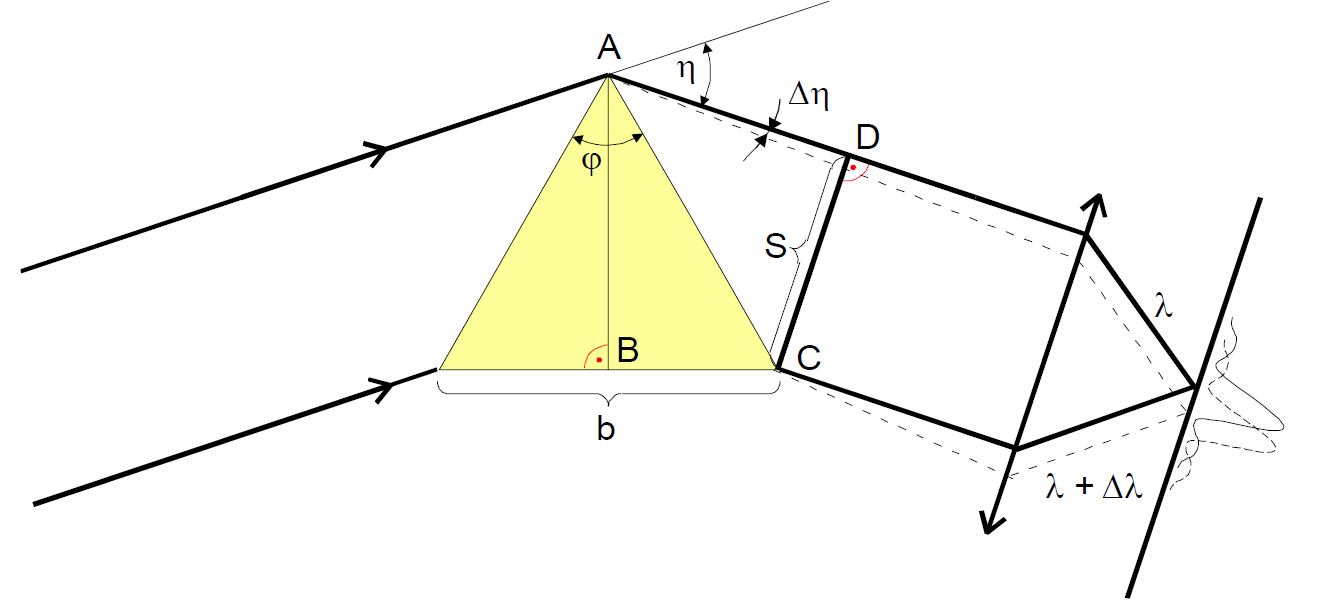
\includegraphics[scale=0.35]{Text/Bilder/Aufloesungsvermoegen.png}
  \caption{Skizze zur Berechnung des Auflösungsvermögens eines idealen Prismen-Spektralapparates \cite[28]{sample}}
  \label{fig:ALV}
\end{figure}
Eine Trennung der beiden Linien soll genau dann noch möglich sein, wenn das Helligkeitsmaximum
einer Beugungsfigur gerade in das erste Minimum der anderen fällt.
Nach längerer Rechnung ergibt sich, dass für das Auflösungsvermögen dann folgender Zusammenhang herschen muss:
\begin{equation}
  A = b\frac{\symup{d}n}{\symup{d}\lambda}\label{eq:A}
\end{equation}

\subsection{Bestimmung des Winkels zwischen den brechenden Oberflächen des Prismas} \label{sec:MessPhi}
Der in Abbildung \ref{fig:Messphi} zu sehende Winkel $\varphi$ lässt sich unter der Annahme, dass die Strahlen parallel auftreffen, mithilfe des Zusammenhangs
\begin{equation}
  \phi = \frac{\phi_r -\phi_l}{2} \label{eq:phi}
  \end{equation}
bestimmen.
\begin{figure}
  \centering
  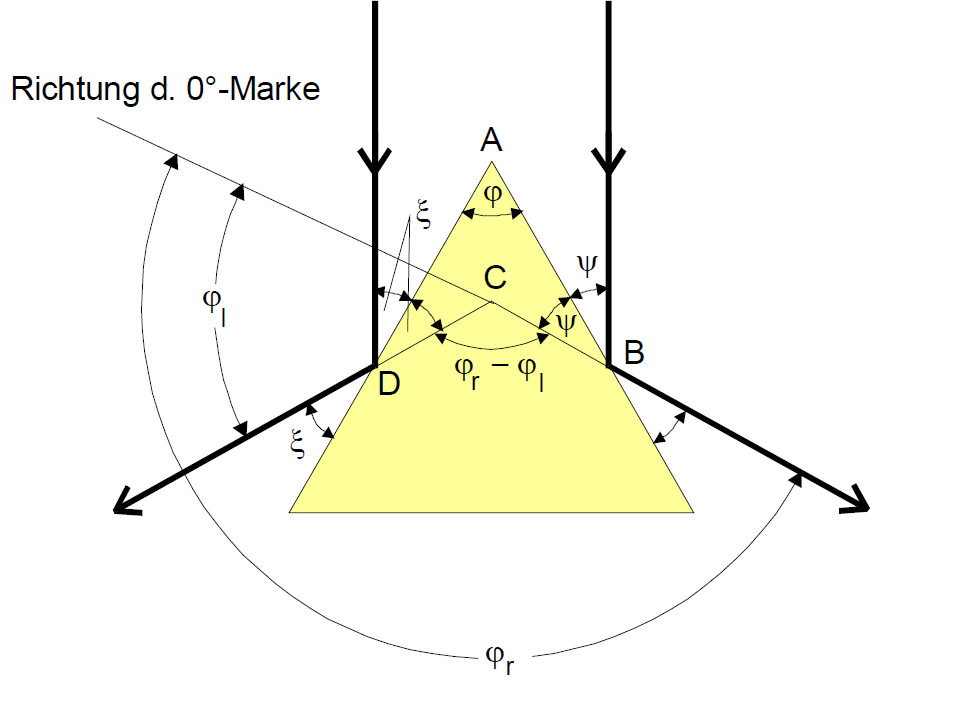
\includegraphics[scale=0.35]{text/Bilder/MessPhi.png}
  \caption{Skizze zur Bestimmung des Winkels $\varphi$ zwischen den brechenden Oberflächen \cite[26]{sample} }
  \label{fig:Messphi}
\end{figure}
Die Winkel $\varphi_r$ und $\varphi_l$ werden im Experiment mithilfe eines Fernrohrs bestimmt, indem die Richtung der reflektierten Strahlen ausgemessen wird.

\subsection{Bestimmung des Brechungswinkels} \label{sec:MessEta}
Der in Kapitel \ref{sec:brech} vorkommende Brechungswinkel $\eta$ lässt sich durch den Zusammenhang
\begin{equation}
  \eta_i = 180\si{\degree}-(\Omega_\text{$r_i$}-\Omega_\text{$l_i$}) \label{eq:eta}
\end{equation} bestimmen.
Dieser Zusammenhang folgt aus geometrischen Überlegungen, die aus den in Abbildung \ref{fig:eta1} und \ref{fig:eta2}zu sehenden schematischen Darstellungen folgen.
\newline
\begin{figure}[H]
  \centering
  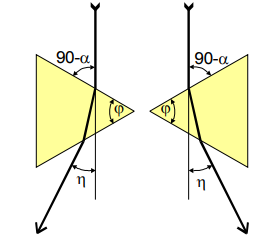
\includegraphics[scale=0.85]{Text/Bilder/MessEta.png}
  \caption{Skizze zur Bestimmung des Brechungswinkels $\eta$ \cite[26]{sample}.}
  \label{fig:eta1}
\end{figure}

\begin{figure}[H]
  \centering
  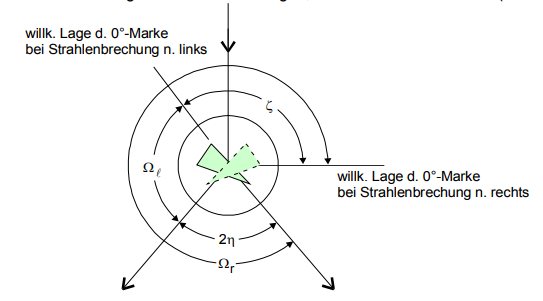
\includegraphics[scale=0.85]{Text/Bilder/MessEta2.png}
  \caption{Darstellung der Messgrößen $\Omega_l$ und $\Omega_r$ in Zusammenhang mit den beiden spiegelbildlichen Prismenstellungen \cite[26]{sample}.}
  \label{fig:eta2}
\end{figure}
